\documentclass{article}

\usepackage[most]{tcolorbox}
\usepackage{physics}
\usepackage{graphicx}
\usepackage{float}
\usepackage{amsmath}
\usepackage{amssymb}


\usepackage[utf8]{inputenc}
\usepackage[a4paper, margin=1in]{geometry} % Controla los márgenes
\usepackage{titling}

\usepackage{accents}
\usepackage{trimclip}

\title{Clase 13 }
\author{Manuel Garcia.}
\date{\today}

\renewcommand{\maketitlehooka}{%
  \centering
  \vspace*{0.05cm} % Espacio vertical antes del título
}

\renewcommand{\maketitlehookd}{%
  \vspace*{2cm} % Espacio vertical después de la fecha
}

\newcommand{\caja}[3]{%
  \begin{tcolorbox}[colback=#1!5!white,colframe=#1!25!black,title=#2]
    #3
  \end{tcolorbox}%
}

\newcommand{\halfapprox}{\clipbox{0em 0em 0em 0.225em}{$\approx$}}

\begin{document}
\maketitle

\section{Variedades Diferenciables}

Vamos a tener x elementos que vamos a describir en coordenadas. Por ejemplo $ x ^ {\alpha } $ o $ y ^ {\alpha} $. Lo que queremos es que la tranformacion entre estas dos coordenadas sean funciones continuas y suaves.

$ M  $ de $ n  $ dimensiones es una variedad diferenciables si: 
\begin{itemize}
  \item $ M  $ es un espacio topológico 
  \item $ u_i  \rightarrow $ abiertos. $ \rightarrow  $ le asociamos unas parejas $ (u_i,\phi_i) $, donde $ \phi_i: u_i \rightarrow \mathbb{R}^ {n } $, esta transformacion debe ser un homeomorfismo.
  \item $ \{u_i\} $ son una cubierta: $ \underset{i \in I }{\cup }U_i = M  $.
  \item Tomemos dos parejas $ U_i, U_j  $ que tengan interseccion $ u_i \cap U_j \neq \emptyset   $. En la variedad $ M  $ va a existir esta interseccion la cual está contenida en ambos conjuntos. La funcion que lleve esta interseccion de $ U_i  $ a $ U_j  $ debe ser diferenciable y suave. Basicamente la condicion 2 nos dice que podemos ir de la variedad diferenciable a $ \phi_i  $ y $ \phi_j  $, mientras que esta condiciones nos dice que podemos ir de $ \phi_i  $ a $ \phi_j  $. 
\end{itemize}

\begin{figure}[H]
  \begin{center}
    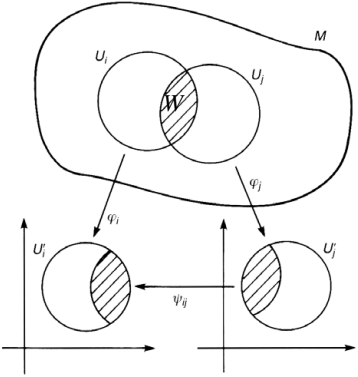
\includegraphics[width=0.3\textwidth]{transformaciones.png}
  \end{center}
\end{figure}

\caja{black}{}{
  \textbf{Charts (cartas)} $ (u_i,\phi_i ) $

  \textbf{Atlas } $ \{(u_i,\phi_i )\} $
}

Si la union de dos atlases $ \{U_i, \phi_i \} $ y $ \{V_i,\psi_i \} $


\subsection{Ejemplos }
\subsubsection{Circulo $ S^1  $}
\begin{figure}[H]
  \begin{center}
    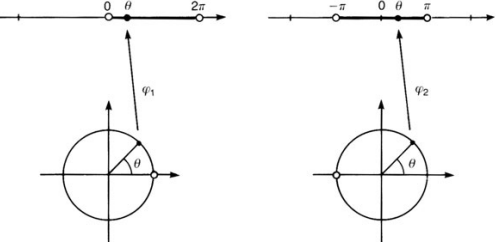
\includegraphics[width=0.5\textwidth]{circulo_s1.png}
  \end{center}
\end{figure}
\begin{gather*}
  \phi_1 ^ {-1 }: (0,2\pi) \rightarrow S^1 \quad \phi_1 ^ {-1 }: \theta \rightarrow (\cos{\theta}, \sin{\theta}) \quad S ^ {1 }-{(1,0)}\\
  \phi_2 ^ {-1 }: (-\pi, \pi ) \rightarrow S ^ {1 } \quad \phi _2 ^ {-1 }: \theta \rightarrow (\cos{\theta}, \sin{\theta}) \quad S ^ {1 }- {(-1,0)}\\ 
  \psi _{12 } ^- = \phi _1 \cdot \phi_ 2 ^ {-1 } \qquad \psi _{21 } = \phi_2 \cdot \phi _1 ^ {-1 } \\
  \text{(Revisar notacion en diapositivas)}
\end{gather*}

Si tomamos un circulo centrado en el origen nos damos cuenta que cada linea corta al circulo en dos puntos.

Tenemos $ \mathbb{R}^ {n+ 1 }:  $Rectas que pasan por el origen. Podemos decir que $ \vec y  $ es proporcional a $ \vec x  $ entonces $ \vec y = a \vec x, \quad a \neq 0  $. Esto lo podemos representar como que este espacion excepto por el 0 es proporcional a la proyeccion de $ \mathbb{R}^ {n } $.
\begin{gather*}
  \{\mathbb{R}^ {n+1 } - \{\vec 0 \}\} / \halfapprox = P \mathbb{R}^ {n }
\end{gather*}

Si $ x ^ {i } \neq 0  $: 
\begin{gather*}
  \xi _{(i)} ^ {k } = \left(\frac{x ^ {0 }}{x ^i }, \frac{x^1 }{x^i }, ..., \frac{x ^ {i-1 }}{x ^ {i }}, \underset{=1 }{\frac{x^i }{x^i }}, ..., \frac{x^n }{x^i }\right)\\
  \xi _{(i) } ^ {k } = \left(\frac{x^0 }{x^i }, \frac{x^1 }{x^i }, ..., \frac{x ^ {i-1 }}{x^i }, \frac{x ^ {i+1 }}{x^i }, ..., \frac{x^n }{x^i }\right)\\
  u_i, \phi_i \qquad \phi_i : u_i \rightarrow \mathbb{R} ^ {n } \qquad u_i : (\vec x )/ x ^ {i }\neq 0 \\
  (x^0,...,x^n) \rightarrow \xi _{(i)} ^ {k }\\
  u_j, \phi_j \qquad \phi_j : (x^0,...,x^n) \rightarrow \xi _{(j)} ^ {k } \qquad u_j : (\vec x )/ x ^ {j }\neq 0 \\
  \psi _{ij }  = \phi _i \cdot \phi_j ^ {-1 }: \quad \phi _j ^ {-1 }[\xi _{(j)} ^ {k }] = x ^ {j }\xi _{(j)} ^ {k } = x ^ {j } \frac{x ^ {k }}{x ^ {j }} = x ^ {k }\\
  \psi _{ij } = \phi _i [\phi_j ^ {-1 }(\xi _{(j)} ^ {k })] = \phi_i (x ^ {k }) = \xi _{(i)} ^ {k } = \frac{x ^k }{x ^i } \quad \text{con }x ^i \neq 0 
\end{gather*}
La funcion $ \phi_i (x ^ {k }) $ es bien comportada ya que $ x^i \neq 0 $.
\caja{black}{}{
  Ver video sobre este tema en el classroom donde se da una descripcion mas geometrica de este problema.
}

\section{Mapas entre variedades }
Vamos a tomar un mapa que va desde la variedad $ M  $ hasta la variedad $ N  $. $ M \rightarrow N  $. La variedad de $ M  $ será $ \mathbb{R}^m  $ y la de $ N  $ será $ \mathbb{R}^n  $. Vamos a tomar un punto $ P  $ de la variedad $ M  $ y lo vamos a llevar hasta $ N  $ utilizando $ f(P)  $. Para esto necesitamos una conexion entre ambas variedades. Osea para establecer un camino de $ \phi (p)  $ hacia $ \psi(f(p)) $ debemos definir un $ f(p)  $ el cual va de $ M  $ hacia $ N  $.

Representación coordenada: 
\begin{gather*}
  y = \psi\circ f \circ \phi ^ {-1 }[x] : \mathbb{R}^ {m } \rightarrow \mathbb{R} ^ {n }\\
  \phi(p) = \{x ^ {\mu }\}, \quad \psi (f(p)) = \{y ^ {\alpha }\}
\end{gather*}

\subsection{Curva $ c  $ en $ M  $}
Vamos a hacer un mapa entre dos variedades pero una de las variedades va a ser un intervalo. 

Vamos a tomar el intervalo $ (a,b) $ y vamos a tomar un punto $ c  $ el cual vamos a llevar hacia la variedad $ M  $ por medio de la funcion $ c  $. Muchas veces este mapeo no está sobre toda la variedad $ M  $ si no sobre una parte de esta, a esta parte la llamaremos $ U  $. Para ir del intervalo hacia la variedad vamos a llamar la funcion $ c(t): \phi \circ c  $: Representación en coordenadas de la curva. 
\begin{gather*}
  c(t) = \phi \circ c : \mathbb{R} \rightarrow \mathbb{R}^ {n } 
\end{gather*}

\subsection{Funcion $ f  $ en $ M  $}
\begin{gather*}
  f: M \rightarrow \mathbb{R}\\
  f \circ \phi ^ {-1 }: \mathbb{R}^m \rightarrow \mathbb{R} \rightarrow \text{Representación en coordenadas de }f.\\
  f(x) = f(\phi ^ {-1 }(x))
\end{gather*}

\subsection{Vector tangente }
Ahora vamos a juntar los dos casos anteriores y definir un vector.

\textbf{Vector} Para definirlo vamos a tomar la curva ya que esta tiene orientación. 

Vamos a definir: 
\begin{gather*}
  \left.\frac{d f[c(t)]  }{d t } \right| _{t=0 }  \quad \rightarrow \quad \text{Derivada de }f \text{ a lo largo de }c. 
\end{gather*}
Notemos que $ f  $ debe ser derivable.
\begin{gather*}
  \left.\frac{\partial f  }{\partial x^i } \frac{d x^i  }{d t} \right|_{t=0} = \left. \frac{d x^i  }{d t } \right| _{t=0 } \frac{\partial f  }{\partial x^i } = X^i \frac{\partial  }{\partial x^i } f \\
      \left. \frac{d f  }{d t }\right| _{t=0 }  = X^i \frac{\partial  }{\partial x^i }f \equiv X[f] \quad \rightarrow \quad X^i: \text{Vector tangente}\\
  X^i = \left.\frac{d x^i  }{d t }(c(t)) \right| _{t=0 } 
\end{gather*}
\caja{red}{}{
  \begin{gather*}
    X \equiv \overset{\text{Componentes}}{X ^ {i }} \underset{\text{Bases}}{\frac{\partial  }{\partial x^i}}
  \end{gather*}
}
Podemos ver $ X^i  $ como las componentes y $ \frac{\partial  }{\partial x^i } $ como las bases.
\begin{gather*}
  \frac{\partial  }{\partial x^i } \equiv e_i \rightarrow \text{Bases coordenadas. } 
\end{gather*}

Si dos curvas pasan por el punto p y tienen la misma tangente se les llama equivalentes.

\end{document}
